\documentclass[tikz,border=10pt]{standalone}
\usepackage{tkz-euclide} % 专门用于几何作图的宏包

\begin{document}

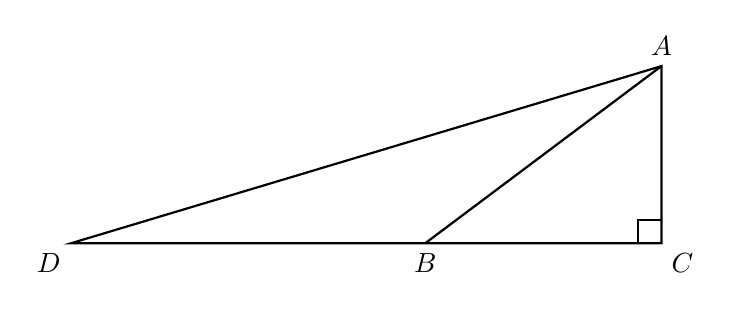
\begin{tikzpicture}[scale=1.5, thick, >=stealth]
    % 1. 定义坐标 (根据原图比例设定参数)
    % C 为直角顶点，设为原点 (0,0)
    \coordinate (C) at (5, 0);
    \coordinate (A) at (5, 1.5);
    \coordinate (B) at (3, 0);
    \coordinate (D) at (0, 0);

    % 2. 绘制主要线段
    \draw (D) -- (C) -- (A) -- cycle; % 绘制大三角形 ADC
    \draw (A) -- (B);              % 绘制斜线 AB

    % 3. 绘制直角标志 (\angle C = 90度)
    \draw (4.8, 0) -- (4.8, 0.2) -- (5, 0.2);

    % 4. 标注点位名称
    % 根据图像位置调整 label 的方向 (node)
    \node[above] at (A) {$A$};
    \node[below] at (B) {$B$};
    \node[below right] at (C) {$C$};
    \node[below left] at (D) {$D$};

\end{tikzpicture}

\end{document}